\subsection{Don't just publish the raw data}

Recall that the main objective of accessing the data is to obtain knowledge, to understand and make sense of it.
Of course, pure data by itself has no value until we can understand it and apply it.
We must contextualize, process, and analyze the information to gain useful knowledge. \\ 
    
\begin{figure}[ht]
    \centering
    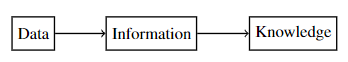
\includegraphics[width=12cm]{Figure_4_3_1_fromDataToInformationDiagram}
    \caption{From Data to Information Diagram}
 \end{figure}
 
\begin{center}
    \bf{        
    Figure 4.3.1. From Data to Information Diagram}
\end{center}
 
In order to obtain this knowledge, the user must correctly interpret the data.
It's not enough to know what the values and units individually represent, but what they mean in the big picture.
For that the user must already have expertise in the area, or must engage in further research allowing them to understand the data that has been extracted.\\
    
In order to build a system that makes data accessible, we need to transform the raw data into a derived model that our users can understand.
For this it will be necessary to have a solid knowledge of the dataset that is needed, the values, their units and how they relate to each other.
The platforms provide a huge volume of data, since, probably they will provide multiple samples containing different sets of fields. 
These field sets may be similar to each other but don't need to be identical.
From this data, we need to select the relevant fields necessary to represent specific model.\\

\subsubsection*{Suggested strategies} 

\begin{itemize}
    \item Design the derived model that can be understood by your users. You may need to use outside expertise to acquire the necessary knowledge on the subject.

    \item Transform the raw data into the derived model, using a series of processes such as extraction, transformation and cleaning of the data.
        Without automation, these processes are tedious and time consuming, so it is strongly advisable for the entire process to be automated.
\end{itemize}

\subsubsection*{In the context of Aire Guru \ldots} 

Aire Guru aims to increase the awareness of the level of pollution that surrounds us.
To do this, it uses a measure called the air quality index (AQI), specifically the European air quality index (EAQI).

\begin{figure}[ht]
    \centering
    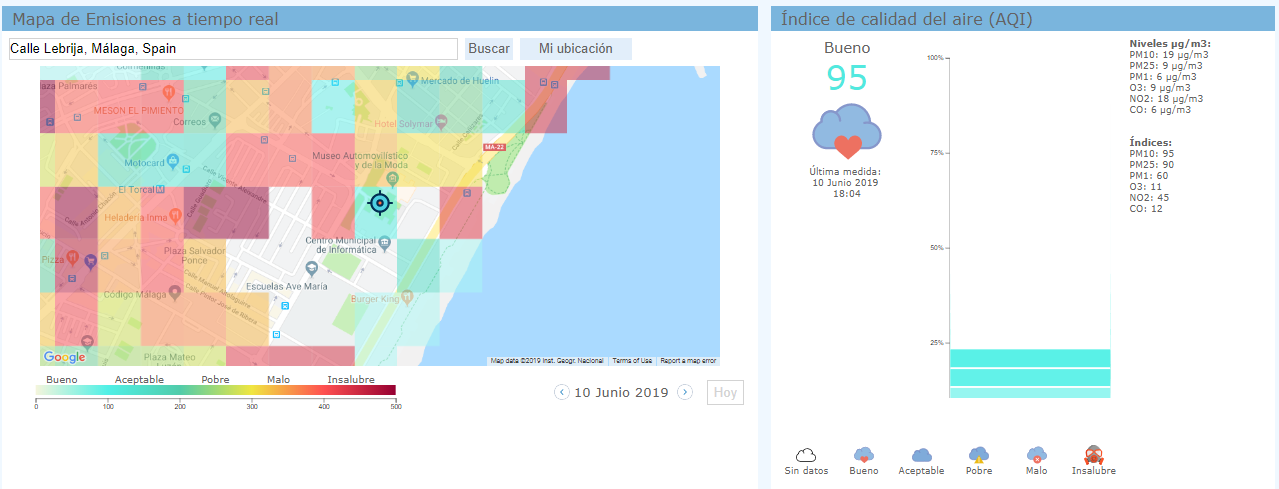
\includegraphics[width=10cm]{Figure_4_3_2_aireGuru_landingPage_topSection}
    \caption{Aire Guru. Landing page. Top section}
\end{figure}
\begin{center}
    \bf{        
    Figure 4.3.2. Aire Guru. Landing page. Top section}
\end{center}

Aire Guru shows the AQI values for the city of Málaga, organized into zones, showing the levels of both the overall pollution and individual pollutants, from September 2018 to the present.
It also shows the evolution of these values in selectable timescales of days, months and years.It is capable of creating a set of the most relevant pollutants for a given medical condition.
An innovative feature is the capacity to display levels of any particular pollutant by hour, day, month, or year. \\

The original source data is in GeoJSON format, a format which provides a JSON object with nested subdocuments.
Each of these subdocuments contains data in key-value form.
In the following figure we can see the beginning of the document downloaded on June 9, 2019 (https://datosabiertos.malaga.eu/recursos/ambiente/calidadaire/calidadaire.json) \\

\begin{figure}[ht]
    \centering
    \subfigure[First subdocument]
        {\centering 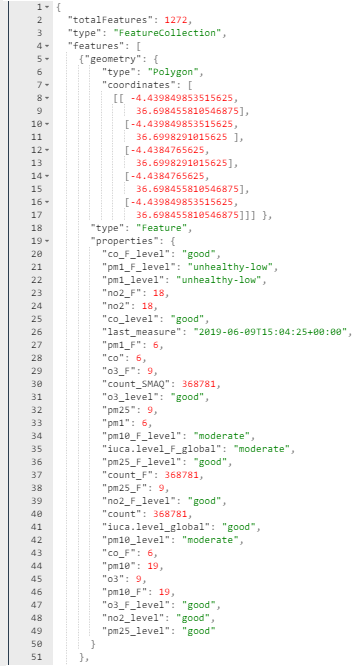
\includegraphics[width=4.75cm]{Figure_4_3_3_a_geoJsonAirQualityData1}}
    \hfill
    \subfigure[Second subdocument]
        {\centering 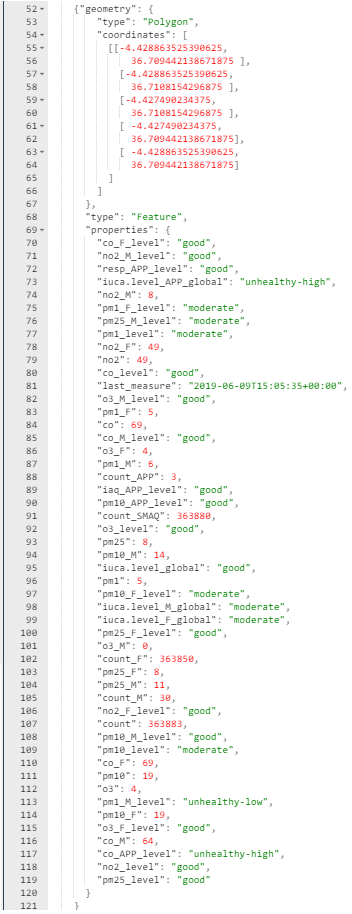
\includegraphics[width=4.75cm]{Figure_4_3_3_b_geoJsonAirQualityData2}}
    \caption{Air quality Document [09/06/2019]. Open Data Portal Málaga}
\end{figure}
    
\begin{center}
    \bf{        (a) First subdocument (b)Second subdocument \\
    Figure 4.3.3. Air quality Document [09/06/2019]. Open Data Portal Málaga}
\end{center}

In the Figure 4.3.3, We can see an excerpt of the first two subdocuments.
Each subdocument contains the coordinates of the air quality measuring station, the date and time when the measurement was recorded, and the values of the measurements.
In the Figure 4.3.4 we can find the description provided by the open data portal.\\
    
\begin{figure}[ht]
    \centering
    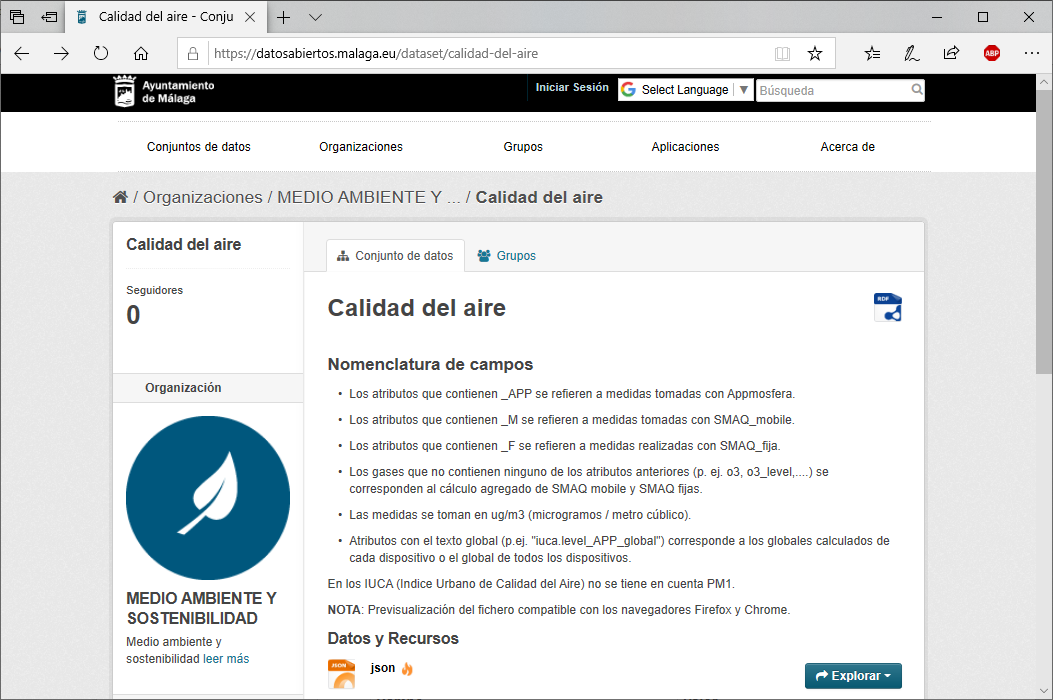
\includegraphics[width=8cm]{Figure_4_3_4_geoJsonAirQualityDataDescription}
    \caption{Air quality data description [09/06/2019]. Open Data Portal Málaga}
\end{figure}
\begin{center}
    \bf{        
    Figure 4.3.4. Air quality data description [09/06/2019]. Open Data Portal Málaga}
\end{center}

For a more detailed description of the measures, we have to resort to an external resource.
In this case we directly contacted the company that installs the UrbanClouds (https://urbanclouds.city/es/) measuring stations and provides the data to the Málaga city council.
After selecting the necessary fields according to our design plan, we carried out sequence of cleaning, transformation and extraction tasks:

\begin{itemize}
    \item \textbf{Cleaning}. We need to eliminate the repeated or non-relevant fields.
        For example, the identifier of the measuring station is unneccessary as the data already contains the coordinates of the station, and coordinate representation is more interesting for our purposes.

    \item \textbf{Transformation}. We need the values to have a format appropriate to the fields that they represent.
        For example, the date and time of the measurement is stored in date format instead of the string provided in the raw dataset.

    \item \textbf{Extraction}. We need to select the relevant fields.
        This dataset offers one or more measurements for each pollutant, which can be represented by three different fields:
        a quantitative measurement, a qualitative of the fixed station of measurement, and a qualitative station of a mobile station.
        We synthesize a field containing the measurement which is most relevant for our purposes, and eliminate the non-relevant values to minimize processing time.
\end{itemize}

For reliability purposes, a second, totally independent process collects and stores the raw data.